% This text is proprietary.
% It's a part of presentation made by myself.
% It may not used commercial.
% The noncommercial use such as private and study is free
% May 2007
% Author: Sascha Frank 
% University Freiburg 
% www.informatik.uni-freiburg.de/~frank/
%
% 
\documentclass{beamer}
\setbeamertemplate{navigation symbols}{}

\usepackage{beamerthemeshadow}


% JW: packages:
\usepackage{amsmath}
\usepackage{graphicx}
\usepackage{fontawesome}
\usepackage{dashrule}
% \usepackage[my options...]{xcolor}:
% NOTE: xcolor is already loaded by beamer.
% When it's loaded with options, compilation will fail.
% If needed, instead before documentclass{beamer} write this:
% PassOptionsToPackage{my options...}{color}.
\usepackage{hyperref}
\hypersetup{
    colorlinks,
    linkcolor={red!50!black},
    citecolor={blue!50!black},
    urlcolor={blue!80!black}
}

% JW: beamer config (can be changed locally)
\setbeamercovered{transparent} % show items in unspecified slides as gray




\begin{document}
\title{SiScLab Project 8}  
\author{Katta, Partmann, Wasmer}
\date{\today} 

\begin{frame}
\titlepage
\end{frame}


\chapter{Introduction}
\label{chap:intro}

\section{Problem Statement}
\label{sec:problem-statement}

%% CP: proofread modification v1 of PK Original ======================================== 
One important problem in solid-state physics is the computation of electronic properties of materials, especially crystals. Since the quantum mechanical equations which describe the physics of electrons in solids are usually impossible to solve with analytical methods, numerical codes were developed to solve these equations efficiently on high-performance computers. The project `Fleur' that this project is based on is a highly optimized code that solves the many-body problem based on the DFT (Density functional theory) approach \cite{fleur}.

Fleur is a freely available full potential linearized augmented planewave (FLAPW) code developed by physicists at the Forschungzentrum Jülich. Like any other kind of numerical simulation, DFT simulations produce a significant amount of data that needs to be preprocessed, visualized and analyzed in order to gain physical insight. 

The whole pipeline, from the raw data generated by Fleur through data exploration to comprehensible plots showing selected physical properties of the simulated material, is addressed in this project. 


% %% PK Original ========================================
% Solid State physics deals with the study of large scale properties of solid materials resulting from the atomic scale properties. A solid state physicist can get to know the atomic scale properties from the experiments conducted on the material. Another way to elucidate physical properties is numerical simulation by means of Density Function Theory (DFT). This method is computational Quantum mechanical modeling method to investigate the electronic structure of many body systems of an atom or molecule. Electron density, Intermolecular forces, charge transfer excitations, calculation of band gap among others are properties that are made amenable by DFT simulations.

% Fleur is one such DFT simulation which is developed by physicists at Juelich Forchungzentrum and most importantly its an open source and anyone can access it and use it. Like any other simulation, DFT simulation also outputs a lot of data for a solid state physicist to understand and determine the properties of a cell structure of a molecule through which physical properties of the material can be determined. Fleur is run specifying the cell structure of a molecule and so can be used on any molecule's cell structure and obtain the characteristics of same.

% Generally it is used to find/simulate properties of solids with impurities in cell structure. Fluer outputs the data of DFT simulation. It gives the data of ground state and excited state properties of solids. These data which are raw are generally not accessible directly and have to be processed through steps for any solid state physicist to understand the raw data extracted from Fleur DFT simulation. This becomes the major problem and which is dealt in this project. The goal of this project was to implement a complete data analysis pipeline for this application. The steps include preprocessing followed by data exploration and visualization.


\section{Motivation and Requirements}
\label{sec:motiv-requ}

%% CP: proofread modification v1 of PK Original ========================================
The main project goal was to develop a software product that is able to perform
all necessary steps of postprocessing including visualization in order to make
the Fleur simulation output easily accessible for both solid-state physicists
and non-experts who use Fleur for the first time alike. 

This imposes several requirements on the software:
\begin{itemize}
    \item Physically accurate and meaningful representation of data: The data reduction strategy during the preprocessing must be transparent and physically motivated. Plots should be in a format well known by any physicist.
    \item Easy to use: The tool must not be overloaded with functionalities for very specific problems, but is supposed to be general and usable in an intuitive way without much explanation.
    \item Easy to access: The tool should be able to run in, or from, different environments with no additional setup.
    \item Reasonably fast: The datasets can be large, therefore efficient preprocessing and plotting techniques are necessary.
    \item Easy to extend and maintain: In order to let the software developed in
        the scope of this project keep pace with external improvements and new
        tools, the code should be written in a modular style.
    \item Export feature: Visualization results have to be exportable as PDF or PNG.
\end{itemize}

The central piece of the project from the physics point of view is the `backend', which is a library that reads the simulation data and prepares it for the visualization. In this module, the dimensionality of data gets reduced according to the choice of the user in a physically meaningful way. The preprocessed data is then passed to a `frontend', that visualizes the preprocessed data. To reach a wide range of potential users, the authors decided to develop a graphical user interface (GUI), where parameters relevant to the visualization can be passed interactively. The visualization produced within this interactive tool can then be exported in order to be shared and discussed.

% %% PK Original ========================================
% An API which solves the physicist's problem of understanding the simulation data which transforms raw data to useful data such that it is process and visualizes. This API has to process the output files from fleur directly so that it is easier for physicists to get the data processed without external effort. Having said this, modularization and easy maintainability of code also matters since the format and structure of simulation results keeps varying over the time with the development of simulation code and more data may be collected from simulation.

% This API shouldn't only be solving the physicist's problem but also should be fast enough in terms of computation. As known, using of computer code to get outputs and may cause confusions in using it as computer code and there is always chance of altering the code while using it. So a front end GUI is needed such that a physicist can use the GUI to input the parameters and to output the processed data. As this is used for research purpose and the features such as plots, images and other should be of high quality and resolution such that there is no uncertainty of the results.


\section{Project Steps}
\label{sec:steps}

%% CP: proofread modification v1 of PK Original
%% ========================================
The project was organized into several steps with the supervisors.
\begin{itemize}
\item Understanding the problem: Understand. the physics of the datasets and how
    the data is used in research. This leads to a list of requirements that the
    software has to fulfill in order to be usable in a productive way.
\item Preprocessing: Write a backend that reads raw data and processes it by transforming it into a format that can be visualized in an efficient way. Therefore, the dimensionality of the data needs to be reduced without losing too much physical information.
\item Exploring the data: Investigate possible challenges that might occur during the visualization of the data. (e.g. how to deal with points/datasets covering each other, ...)
\item Visualization: The preprocessed data is visualized in a scatter plot with
    a format well known in the physics community.
\item Frontend: A GUI with intuitive features is developed such that a wide
    range of users can access Fleur output without having to deal with the raw data. 
\item Test the usability of the software using typical Fleur output files. Prove that physical insight can be gained easily using the software.
\item Deployment: Bring the project into a form that can be distributed.
\end{itemize}


% %% PK Original ========================================
% The project steps by step procedure has completed to complete the task of processing and visualization.
% \begin{itemize}
% \item Understanding the problem: Firstly the theory of DFT simulation, Fleur code, band plots, density plots, file format of data and other necessary theory needed are learnt and problem of the project to process the data in different steps is understood.
% \item Pre-Processing: Once problem is clearly understood, first step of project comes to preprocessing the data. Reading the data, sorting the data and storing it sorted which can be used in further stages of implementation.
% \item Exploring the data: From the raw data, not just band plots but many features can be extracted. Finding out the features through exploring the data and trying to understand and extract those features is done.
% \item Visualization: The data which is pre-processed and extracted need to be visualized into plots such that any user with solid state physics background can understand it with an observation.
% \item Front End: A GUI is developed so that its easier in future for any physicist to just run the GUI and get the plots and other visualization instead going through hassle of code and letting a chance of code being disturbed unintentionally
% \item Results and lookup: Getting to know the features extracted, studying it,
%     reporting the same.
% \end{itemize}




%%% Local Variables:
%%% mode: latex
%%% TeX-master: "../"
%%% End:

%  LocalWords:  frontend


\chapter{Theoretical Background}
\label{chap:theory}

%...some introduction scentence depending on intro chapter...

%The visualization pipeline developed in this project is supposed to process data that is produced by the scientific code Fleur \cite{fleur}.

Fleur computes the electronic structure in crystals using the density functional theory approach (DFT), which is one of the state of the art method for this problem. The many-body Schrödinger equation, that can be used to describe electrons in solids, is almost impossible to solve directly, because the storage of the wavefunctions of each of the $N$ electrons in the system at each spatial coordinate exceeds the memory of any currently available computer for even quite small $N$. This motivates the DFT approach, that uses two fundamental theorems to reduce the computational complexity of the many-body problem significantly: The Hohenberg-Kohn theorem \cite{hohenberg-kohn} allows to use the electron density instead of the $N$-electron wavefunctions to uniquely characterize the ground state of a system. With the Kohn-Sham equations \cite{kohn-sham}, the interacting Hamiltonian of the system can be replaced by non-interacting equations with an effective potential. This so-called KS-DFT approach reduces the dimensionality of the problem from $N^3$ to $3$ and trades the interacting Hamiltonian for a set of non-interacting equations that have to be solved self-consistently. In general, the DFT approach is not just limited to computations of electrons in crystals, but is also for example used in chemistry to compute nonperiodic molecules.
% 
The output of a DFT calculation includes various physical quantities, for instance, the three-dimensional spatial electron density, which is the central quantity in DFT calculations. In this project, however, we focus on two quantities that are easy to interpret, already reduced in dimensionality and frequently used in both experimental and theoretical physics.

The band structure $E(\mathbf{k})$ represents the eigenenergies of the eigenfunctions of the Hamiltonian for each crystal momentum $\mathbf{k}$. It is the dispersion relation of electrons in the crystal and relates allowed momenta and energies. In general, $E(\mathbf{k})$ is defined at any point inside the Brillouin zone, which is a special choice of the unit cell in the reciprocal lattice of the crystal. Both, the real space lattice and the reciprocal lattice are shown for a face-centered cubic (fcc) crystal in figure \ref{fcc}. For larger unit cells with fewer symmetries, the Brillouin zone can be much more complicated than in the shown example. In order to reduce the dimensionality of $E(\mathbf{k})$ with $k \in {\rm I\!R}^3$, the dispersion relation is only sampled along a discrete one-dimensional path between high symmetry points in the Brillouin zone. This path still contains most of the relevant physical features.

\begin{figure}[htb!]
    \centering
    \begin{subfigure}{.5\textwidth}
        \centering
        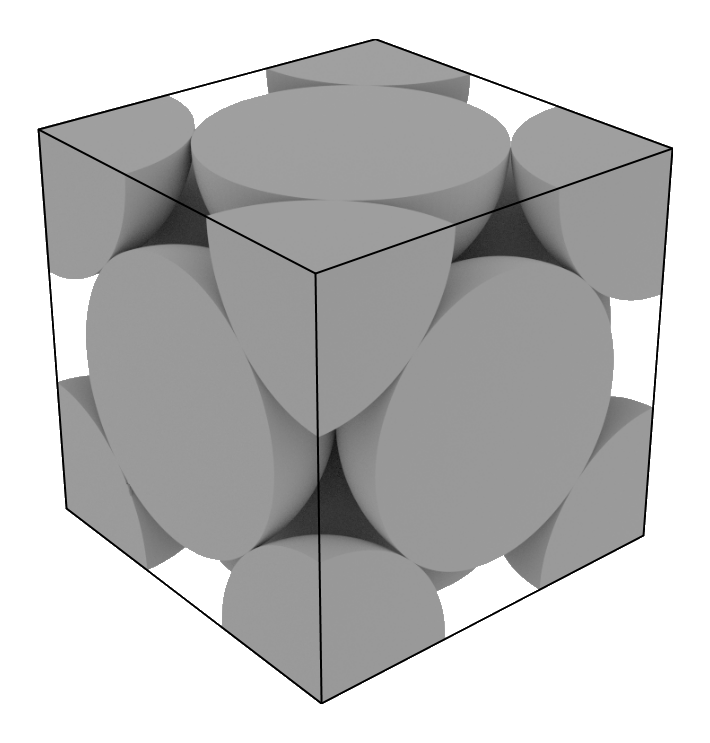
\includegraphics[width=0.5\linewidth]{christian/fcc_real.png}
        \caption{Lattice in real space}
        \label{fig:fcc_real}
    \end{subfigure}% %this '%' is needed for side-by-side figure!
    \begin{subfigure}{.5\textwidth}
        \centering
        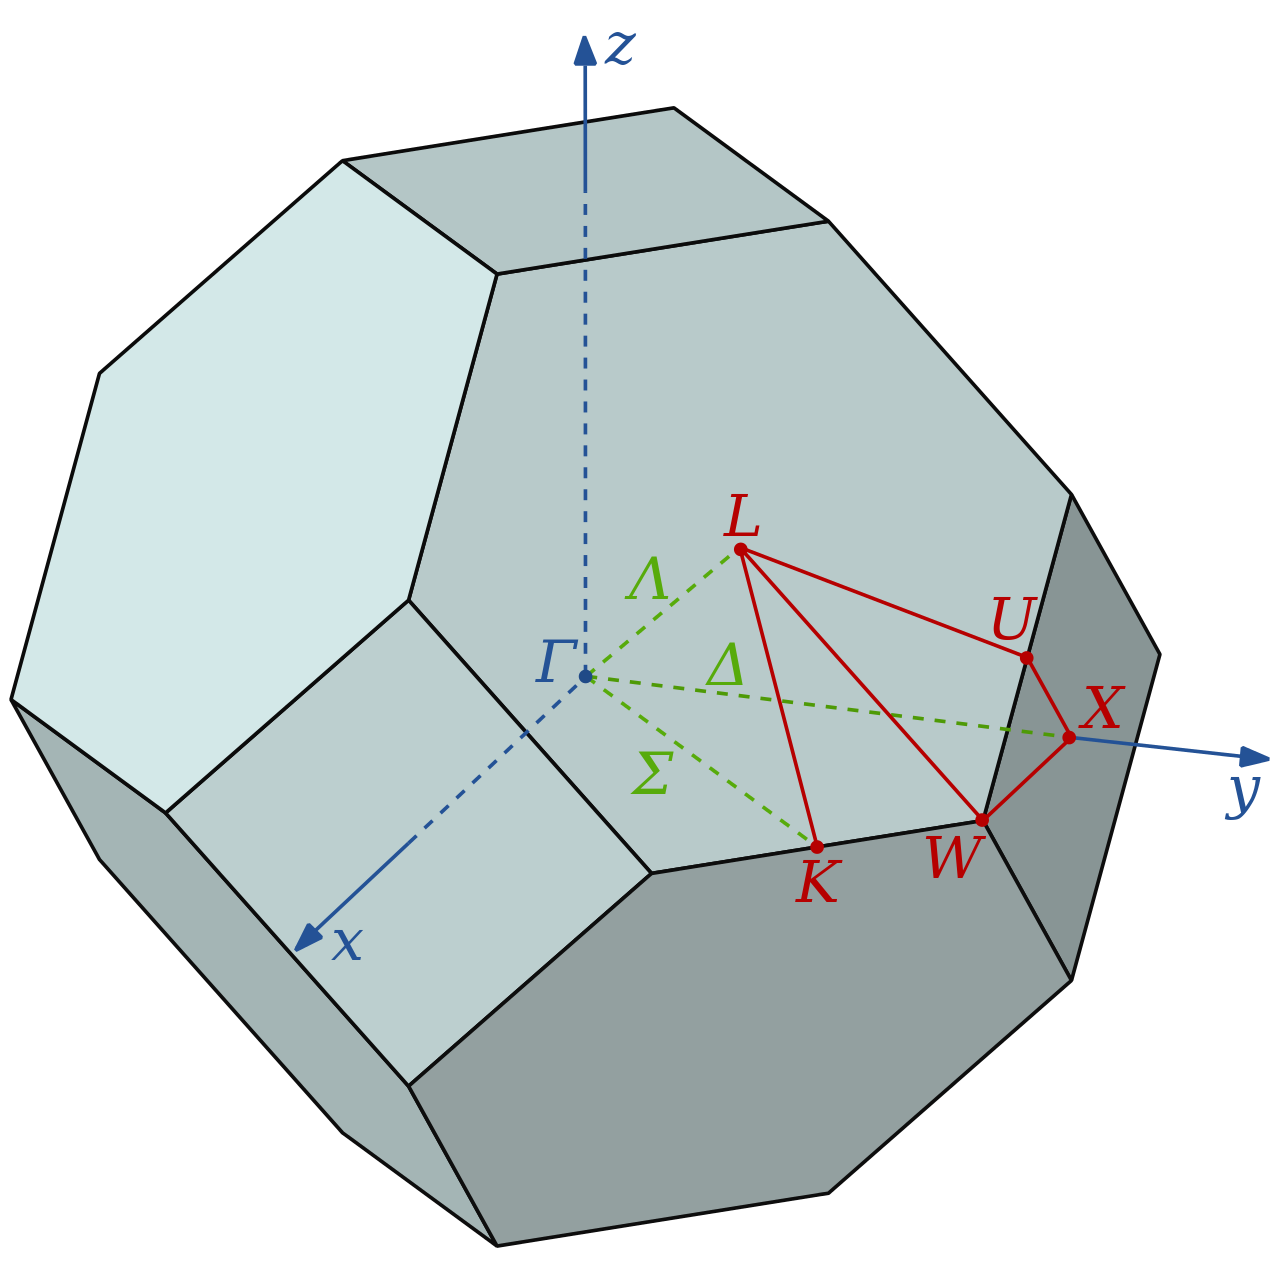
\includegraphics[width=0.5\linewidth]{christian/Brillouin_Zone_(1st,_FCC).png}
        \caption{Brillouin zone}
        \label{fig:fcc_billouin}
    \end{subfigure}
    \caption[Brillouin zone of an fcc lattice]{Brillouin zone of an fcc lattice. The red curve in the reciprocal lattice represents a possible sampling path of $E(\mathbf{k})$ in the reciprocal lattice.}
    \label{fcc}
\end{figure}

The second central quantity in this project is the density of states (DOS)
$D(E)$, which describes the number of states per energy interval that is
independent of the crystal momentum. In this sense, the DOS is also derived from
$E(\mathbf{k})$, but instead of just selecting a subset, the $\mathbf{k}$
dependency is summed out. This sum is performed internally by Fleur, since
$E(\mathbf{k})$ must be known at every grid point in the Brillouin zone. Both complementary quantities together are a common choice for comprehensive visualizations of electronic structure data while still capturing most of the important physics. 

For applications, it is useful to investigate where the contributions to $E(\mathbf{k})$ and $D(E)$ come from. Therefore, the data contains the weights of each basis function of the DFT calculation belonging to the individual atom groups and the orbitals. This means that spatial information about the system can be restored by considering only contributions from certain atom groups. (An atom group contains all atoms that are equivalent with respect to symmetries of the real space lattice.) On the other hand, the projection on the (hydrogen-type) orbitals s, p, d, f encode information about the shape of the wavefunction at each atom. These contributions are stored in the form of relative weights that can be summed to include contributions for multiple groups and orbitals. In case of distinct spins in the crystal, $E(\mathbf{k})$, $D(E)$ and the weights can be different for both spins and are therefore stored individually.



%%% Local Variables:
%%% mode: latex
%%% TeX-master: "../report"
%%% End:


\chapter{Implementation}
\label{chap:implementation}
% logo definitions
\newcommand{\logoFleur}{%
  \begingroup\normalfont
  
\includegraphics[height=1.2\fontcharht\font`\B]{img/logo/fleur.png}%
  \endgroup
}
\newcommand{\logoAiida}{%
  \begingroup\normalfont
  
\includegraphics[height=1.0\fontcharht\font`\B]{img/logo/aiida.png}%
  \endgroup
}
\newcommand{\logoAiidalab}{%
  \begingroup\normalfont
  
\includegraphics[height=1.0\fontcharht\font`\B]{img/logo/aiidalab.png}%
  \endgroup
}
\newcommand{\logoBinder}{%
  \begingroup\normalfont
  
\includegraphics[height=1.2\fontcharht\font`\B]{img/logo/binder.png}%
  \endgroup
}
\newcommand{\logoBokeh}{%
  \begingroup\normalfont
  
\includegraphics[height=1.2\fontcharht\font`\B]{img/logo/bokeh.png}%
  \endgroup
}
\newcommand{\logoDash}{%
  \begingroup\normalfont
  
\includegraphics[height=1.2\fontcharht\font`\B]{img/logo/dash.png}%
  \endgroup
}
\newcommand{\logoDocker}{%
  \begingroup\normalfont
  
\includegraphics[height=1.2\fontcharht\font`\B]{img/logo/docker.png}%
  \endgroup
}
\newcommand{\logoHoloviews}{%
  \begingroup\normalfont
  
\includegraphics[height=1.2\fontcharht\font`\B]{img/logo/holoviews.png}%
  \endgroup
}
\newcommand{\logoHvplot}{%
  \begingroup\normalfont
  
\includegraphics[height=1.2\fontcharht\font`\B]{img/logo/hvplot.png}%
  \endgroup
}
\newcommand{\logoJavascript}{%
  \begingroup\normalfont
  
\includegraphics[height=1.2\fontcharht\font`\B]{img/logo/javascript.png}%
  \endgroup
}
\newcommand{\logoJupyter}{%
  \begingroup\normalfont
  
\includegraphics[height=1.2\fontcharht\font`\B]{img/logo/jupyter.png}%
  \endgroup
}
\newcommand{\logoMatplotlib}{%
  \begingroup\normalfont
  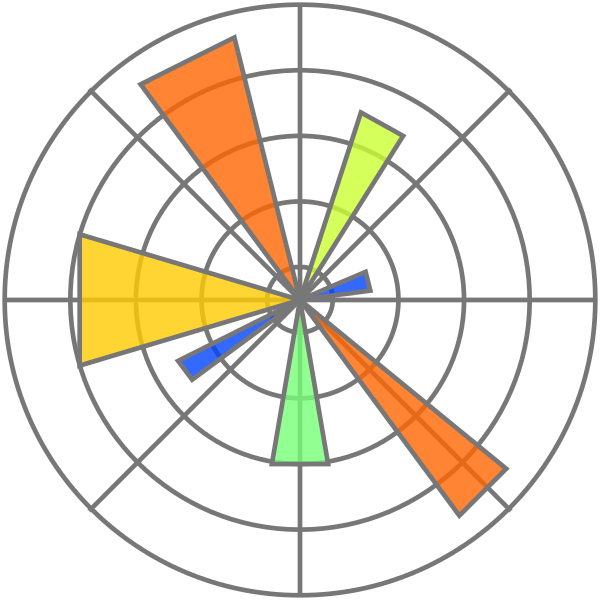
\includegraphics[height=1.2\fontcharht\font`\B]{img/logo/matplotlib.png}%
  \endgroup
}
% \newcommand{\logoMpld3}{%
%   \begingroup\normalfont
%   
\includegraphics[height=1.2\fontcharht\font`\B]{img/logo/mpld3.png}%
%   \endgroup
% }
\newcommand{\logoPanel}{%
  \begingroup\normalfont
  
\includegraphics[height=1.2\fontcharht\font`\B]{img/logo/panel.png}%
  \endgroup
}
\newcommand{\logoParam}{%
  \begingroup\normalfont
  
\includegraphics[height=1.2\fontcharht\font`\B]{img/logo/param.png}%
  \endgroup
}
\newcommand{\logoPlotly}{%
  \begingroup\normalfont
  
\includegraphics[height=1.2\fontcharht\font`\B]{img/logo/plotly.png}%
  \endgroup
}
\newcommand{\logoPython}{%
  \begingroup\normalfont
  
\includegraphics[height=1.2\fontcharht\font`\B]{img/logo/python.png}%
  \endgroup
}
\newcommand{\logoPyviz}{%
  \begingroup\normalfont
  
\includegraphics[height=1.2\fontcharht\font`\B]{img/logo/pyviz.png}%
  \endgroup
}
\newcommand{\logoSeaborn}{%
  \begingroup\normalfont
  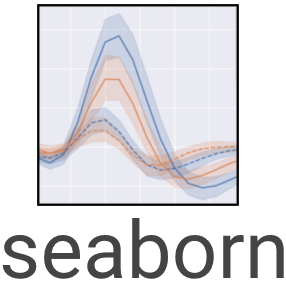
\includegraphics[height=1.2\fontcharht\font`\B]{img/logo/seaborn.png}%
  \endgroup
}

%%% Local Variables:
%%% mode: latex
%%% TeX-master: t
%%% End:


As per the requirements expounded upon in the introduction, the deliverable of
the project should be a finished software product. The software is written in
Python so as to integrate easily with the research group's ongoing software
projects around the Fleur code \cite{fleur}. These are chiefly the group's
materials science tool collection \texttt{masci-tools} \cite{masci-tools} ,
where also this project's code is hosted, and the 'Automated Interactive
Infrastructure and Database for Computational Science' (AiiDA) \cite{aiida}. The
product stakeholders split into frontend users and code developers. In order to
accommodate this, the product is organized into three unidirectionally dependent
subpackages or -modules, see Figure \ref{fig:submodules}.

An important design consideration was to account for unknown use cases. This has
been realized in each submodule by the decoupling of \textbf{interface} and
\textbf{implementation}. The interfaces do not rely on any specific input file
format, visualization method or package, unlike the implementations for a
specific task or \textbf{application}. The word 'application' in this section
denotes the band structure and density of states visualization, and for these,
implementations are provided.

This design choice was also one reason why the product does not reuse any of the
\texttt{masci-tools} routines which partly solve quite similar problems, but
seemed to be too specialized in an cursory code review. For these developers,
one added value of the project product could be to inspire the hopefully easy
integration into a common interface, where the current abstraction level could
serve as a starting point.

%% Bad: jumbles up text
% \begin{wrapfigure}{r}{0.3\textwidth}
%     \centering
% \end{wrapfigure}

%% bad: too near to page side margins
% \begin{figure}[htb!]
%     \centering
%     \begin{subfigure}{.5\textwidth}
%         \centering
%         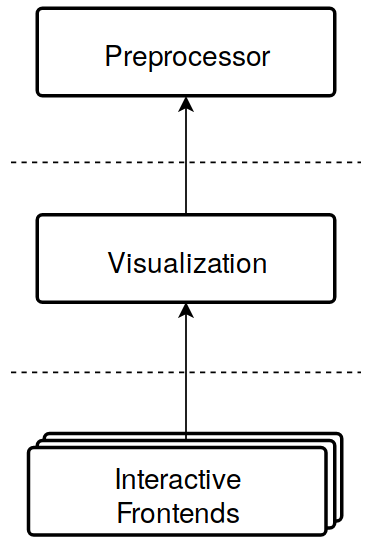
\includegraphics[width=0.5\textwidth]{img/module_design.png}
%         \caption{Submodules}
%         \label{fig:submodules}

%     \end{subfigure}% %this '%' is needed for side-by-side figure!
%     \begin{subfigure}{.7\textwidth}
%         \centering
%         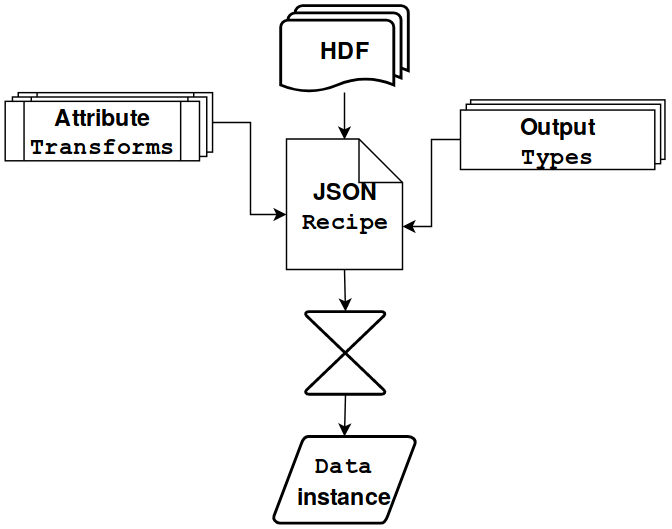
\includegraphics[width=0.7\textwidth]{img/reader_flowchart4.png}
%         \caption{Preprocessor}
%         \label{fig:preprocessor}
%     \end{subfigure}
%     \caption{Module Design.}
%     \label{fig:module-design}
% \end{figure}


\begin{figure}[htb!]
    % Fixed length
    \centering
    \subcaptionbox{Submodules\label{fig:submodules}}{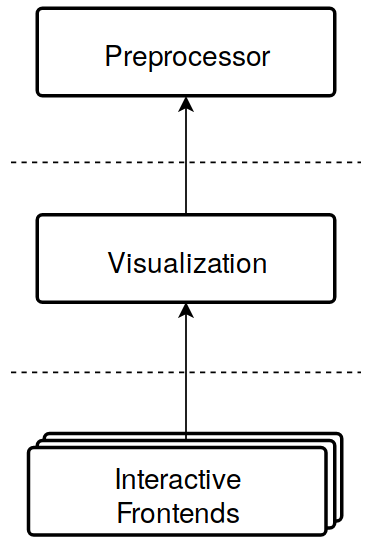
\includegraphics[width=1.6in]{img/module_design.png}}\hspace{5em}%
    \subcaptionbox{Preprocessor\label{fig:preprocessor}}{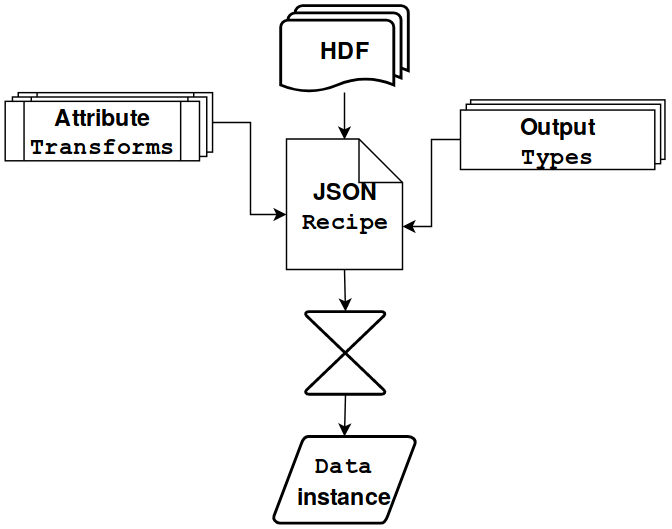
\includegraphics[width=0.5\textwidth]{img/reader_flowchart4.png}}
    \caption{Module Design.}
    \label{fig:module-design}
\end{figure}


\section{HDF Preprocessor Module}
\label{sec:preprocessor-module}

\subsection{Interface}
\label{sec:preprocessor-interface}

This is the 'backend' of the tool. It is basically a file reader for the input
data, for example a Fleur simulation output. Supported formats are the
Hierarchical Data Format (HDF) \cite{hdf} for the band structure, and a simple
Fleur-specific comma-separated values (CSV) format for the density of states
(DOS).

The HDF format is basically a binary flexible container for all kinds of common
binary and text file formats, each of which constitutes a \texttt{Dataset}
inside the HDF file. The format supports metadata annotation and high-throughput
input/output (I/O). As a consequence, it is considered by some developers in
some application domains relying on numerical simulation codes, to be one
possible base for the establishment of common domain-specific rich data exchange
standards in order to increase code interoperability. These developers are in
the process of extending their codes' I/O capabilities towards that end.
However, HDF's flexibility comes at the price of a relatively complex Application
Programming Interface (API) as the keyhole for all operations.

The preprocessor module tries to hide that complexity by offering the
\texttt{Recipes} interface, see Figure \ref{fig:preprocessor}. A specific
application \texttt{Recipe} is a dictionary that aims to describe a complete
\href{https://en.wikipedia.org/wiki/Extract,_transform,_load}{Extract-Transform-Load}
(ETL) pipeline for one specific application. The 'extract' is the reading of a
dataset from HDF, the 'transform' a sequence of once-through functions applied
to the the dataset, and the 'load' the aggregation of all transformed datasets
into one runtime object that has all the methods for operations on the data that
are going to be used later on in the intended application.

The 'transform' and 'output' type methods are defined in hierarchical
\texttt{Transform} and \texttt{Output\_Type} classes, which sort them from
general to application-specific applicability. This structure is built using
Python's \texttt{AbstractBaseClass} (\texttt{ABC}) interface and multiple
inheritance. The advantages of the 'Recipes approach' are:
\begin{itemize}
\item All ETL processes for one application are collected in one simple list
    (the recipe), not locked in different code locations with conflicting
    contexts. In this list, entries can be sorted in any manner, e.g.
    alphabetical for perusal. Thus a recipe also serves as a concise
    documentation of how an application-domain HDF format expects to be handled.
\item Recipes are de/serializable (can be read from and saved to disk) and thus be
    created and manipulated by code.
\item The ETL processes declared in this way can be easily reused across
    applications. A recipe can combine different output types into a new type.
\end{itemize}

The feature that enables this flexibility is \textbf{type introspection}: the
preprocessor processes the datasets listed in the recipe in the order of their
mutual dependencies as found in the used transform and output methods. When all
transformed datasets have been added to the object, all specified output types
are searched and all their methods and attributes added. Thus the output
object's type is defined at runtime, when the preprocessing is finished.

% \begin{figure}[htb!]
%     \centering
%     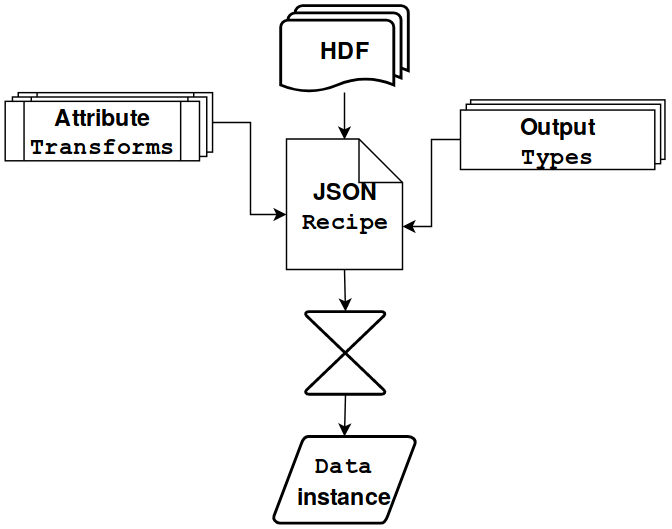
\includegraphics[width=0.6\textwidth]{img/reader_flowchart4.png}
%     \caption{The preprocessor module.}
%     \label{fig:preprocessor}
% \end{figure}

% \lstinputlisting[
% language=python,
% style=code,
% linerange=101-106
% captionpos=t,
% caption={Recipe \texttt{FleurBands} excerpt: dataset \texttt{BravaisMatrix}},
% label=recipe
% ]{listings/recipes.py}


\subsection{Implementation for Band Structure Visualization}
\label{sec:preprocessor-implementation}

\textbf{TODO} describe how bandstructure data is preprocessed for visualization
including user selections AND optimizations

The frontend has to draw three kinds of plots: a 3D atom plot of the unit cell
or supercell, and a combined band structure and DOS plot sharing the same
vertical energy axis. If no DOS data is present, the DOS plot will be omitted.
All three plots are controlled by one set of widgets for varying the parameters.
In the current implementation, the data for the first two plots come from a HDF
file, while the data for DOS plot come from CSV files.

The band structure plot is a scatter plot and plots discrete \(E(\mathbf{k})\) data
from the simulation. It first needs the \(k\)-path (where \(|\mathbf{k}|=k\)) for
the horizontal axis. The preprocessor, having received the recipe
\texttt{FleurBands}, computes it from the \(k\)-points in the HDF in a
transform. Next, the plot needs the eigenergies for every point on the
\(k\)-path, labeled by the band index \(\nu\), and its associated \(l\)-like
charge \(n_{s,k,\nu,g,l}\). It is fivedimensional, and represents the
contribution of spin \(s\), point \(k\) point on \(k\)-path, band \(\nu\), atom
group \(g\), and character or orbital \(l\) (here: only s,p,d,f) to the specific
eigenergy. In order to visualize this, resolves the processed data into the
like-named output type \texttt{FleurBands}. This type has a data filter method.
The respective \texttt{BandPlot} type calls this filter with a user selection of
subsets of all \((s,k,\nu,g,l)\). The method then computes the according
\textbf{effective weight} shown in Equation \ref{eq:effective-weight}. This is
used for the dot size of each \(E(k)\) in the plot. Before rendering, the
plotter normalizes the energies to the Fermi Energy.

\begin{align}
  W^{\text{eff}}_{s,k,\nu} = \left( \frac{\sum\limits_{\substack{g \in \text{groups} \\ l \in \text{characters}}} n_{s,k,\nu,g,l}\, N_g}{\sum\limits_{\substack{g \in \text{all groups} \\ l \in \text{all characters}}} n_{s,k,\nu,g,l}\, N_g} \right) \left(W_{s,k,\nu}^{\text{unf}}\right)^\alpha
\label{eq:effective-weight}
\end{align}

\(N_g\) denotes the number of atoms in a group. \(W_{s,k,\nu}^{\text{unf}}\) is
the unfolding weight and \(\alpha\) its exponent. The effect of unfolding is
illustrated in Figure \ref{fig:unfolding} for a toy example of a monatomic
chain, with a two-atom supercell of size \(a'\) representing \(\alpha=0\) and a
one-atom unit cell of size \(a\) representing \(\alpha=1\). A use-case is
discussed in the Application Chapter \ref{chap:applications}.

\begin{figure}[htb!]
    \centering
    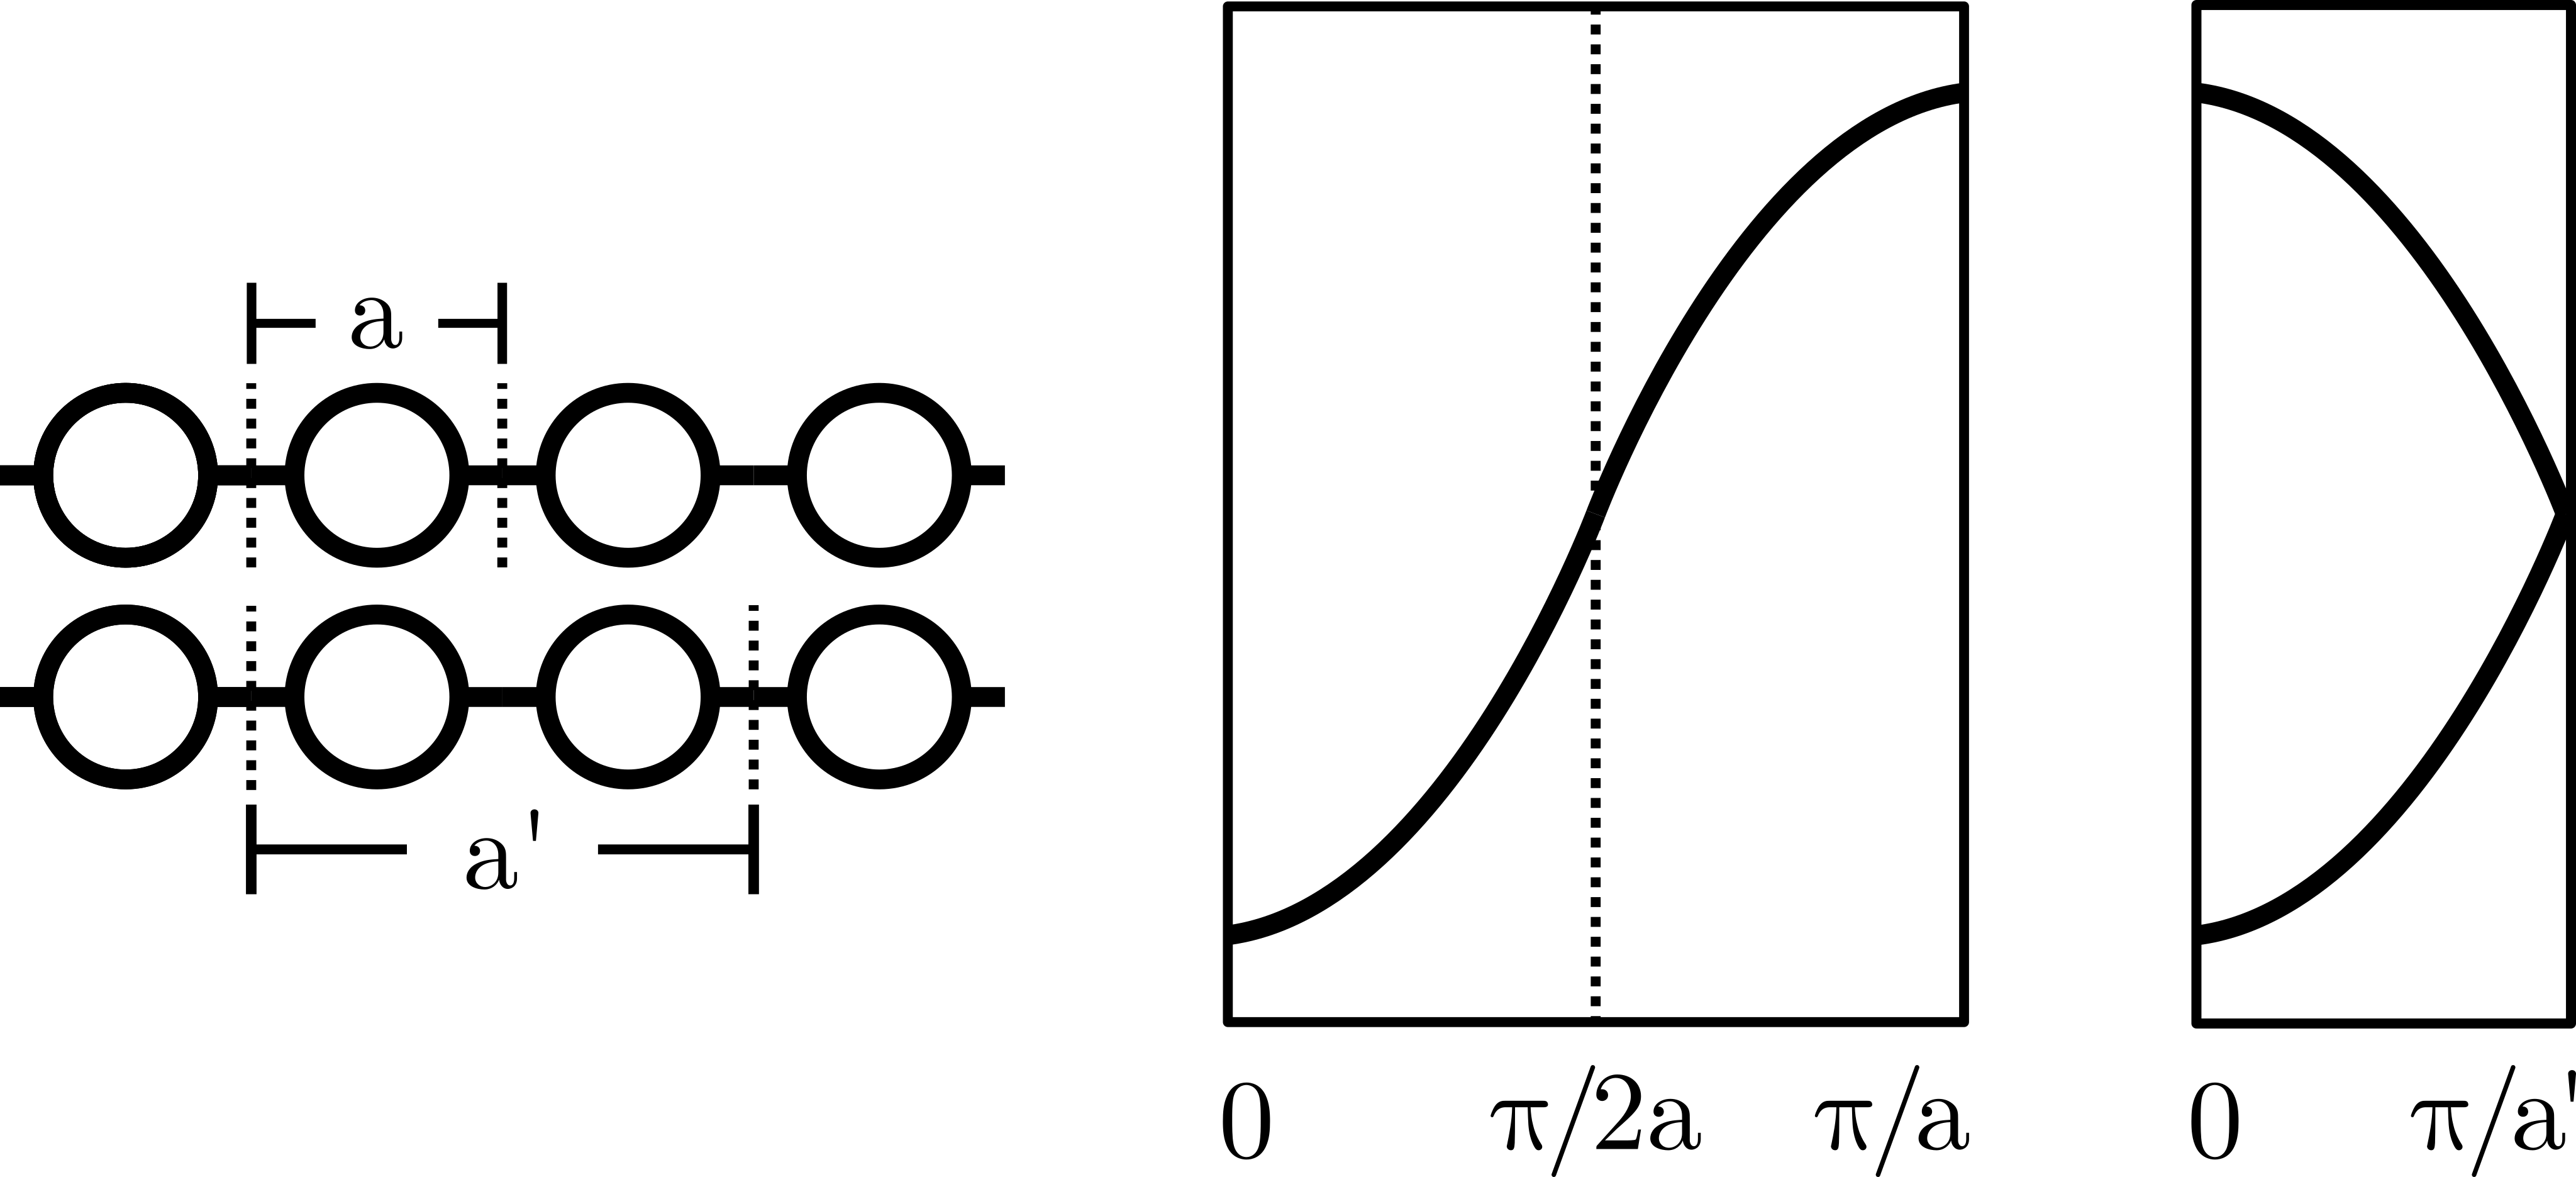
\includegraphics[width=0.6\linewidth]{fig/unfolding.png}
    \caption[Band Unfolding]{Band Unfolding: Example for a simple monatomic
      chain \cite{hoffmann1987chemistry}.}
    \label{fig:unfolding}
\end{figure}

Even for small band structures, the filter has to access on the order \(10^7\)
individual data points for every selection change. Optimizations were introduced
which included: a cutoff skipping effective weights too small,use of optimized
Numpy functions like \texttt{np.tensor}, data buffering, and array reshaping.
Together, these achieve a speedup of approximately \(10^2\) in plotting speed.
Thanks to that, the tool remains usable even when input data is in the \(10^2\)
MB range.

\section{Visualization Module \& Interactive Graphical Frontends}
\label{sec:visualization-module}

\textbf{TODO} Frontends: combine into one subsection when finished. usage will
be in user manual next section.

\subsection{Visualization Module}
\label{sec:visualization-interface}

The Python visualization landscape abounds with a rapidly evolving plethora of
plotting libraries for different application contexts and technology stacks
\cite{python-viz-landscape}. Thus the project's visualization module first
design objective was to account for that by decoupling from specific library
use, and modularizing applications. This structure again is built using Python's
\texttt{AbstractBaseClass} (\texttt{ABC}) interface and multiple inheritance.
Each application is represented by an abstract base class that contains the
common plotting method signatures. Each plotting library is represented by an
abstract base class that contains library-specifics. An implementation inherits
both from one library base class and one or more application base classes. See
Fig. \ref{fig:visualization-module} for an impression. Thus switching the
library in a frontend should require minimal adjustment, and a new application
can be build using existing ones.

The second design objective was for the plotting methods to to hide all
interactions with the actual plotting library used under the hood, while the
method arguments only relate to the preprocessed data being plotted. Thus
different frontend implementations only all call one common method for one
specific plot and receive the identical visualization with identical interactive
behavior.

\begin{figure}[htb!]
    \centering
    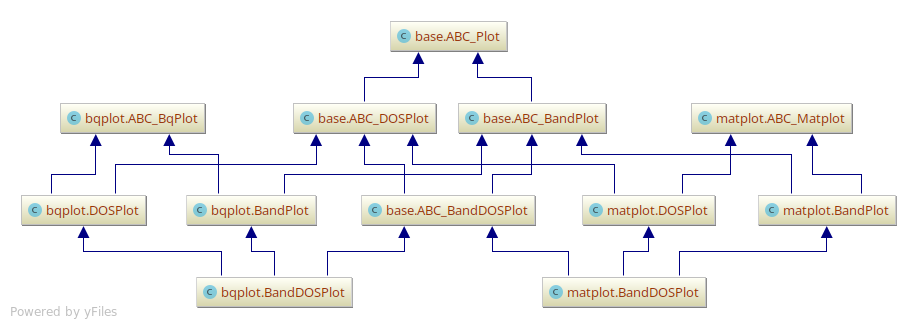
\includegraphics[width=1.0\linewidth]{img/pycharm_uml/matplot.png}
    \caption[Visualization Module Design]{Visualization Module Design: Example
      Structure for two applications \texttt{BandPlot} and \texttt{DOSPlot}, and
      two plotting libraries \texttt{matplotlib} and \texttt{bqplot}.}
    \label{fig:visualization-module}
\end{figure}

\subsection{Desktop Frontend}
\label{sec:desktop-frontend}

A Desktop Frontend is always a helping had for the physicists to just run it on the computer when one wants to go through the plots of the raw data that is already in computer. 
Since the reading of HDF files and preprocessing of the data is done using Python, it is decided that it would be better to use python for front end development. Considering various packages for front end in python such as PyQt, Tkinter and other packages available for Desktop frontend, the conventional tkinter is selected based on the maintainability of the code. It is a package where every button can be designed and can be assigned to function.
Functions like label, button, checkbutton, listbox, canvas for plots, tab for viewing each plot in different tab are used to make a simple Desktop front end. It is simple to use with limited options of what any physicist needed and also easy to convert it into a executable software and run in any system without any installation.

\subsection{Web Frontend}
\label{sec:web-frontend}

As Web Frontends increasingly replace traditional Desktop Frontends in the
modern software environment \cite{web-vs-desktop}, so Python-based Frontends and
visualizations are increasingly moving towards the browser. There, GUIs with
interactive visualizations are often called \textbf{Dashboards}. In the project
context, a survey was undertaken in order to choose the most suitable technology
stack. The full survey is documented in \cite{jw-notes}. The requirements for
the solution stack, added to those in the introduction, were as follows:

\begin{enumerate}
\item \textbf{openness}: relies solely on Open-Source-Software (OSS) with
    licensing suitable for academic use, sports a stable release cycle, developer
    base and documentation,
\item \textbf{dashboarding}: features graphical control elements (widgets) that
    interact with InfoVis\footnote{InfoVis libraries: visualizations of
      information in arbitrary spaces, not necessarily the three-dimensional
      physical world. Example: matplotlib. SciVis libraries: visualizing
      physically situated data. Example: VTK \cite{python-viz-2018}.} plotting
    libraries,
\item \textbf{deployment}: ideally works like any web service, i.e. only a
    modern web browser is required to use it,
\item \textbf{maintenance}: requires only Python and no Web Development
    knowledge like e.g. Javascript, with respect to the product stakeholders.
\end{enumerate}

The last point implies a client-server model where the dashboard app is hosted
by a remote service. This model requires a communication framework and protocol
between the Python interpreter running on the server and the JavaScript
interpreter running in the client browser. As per requirement number two, unlike
a generic Python web framework like e.g. \href{http://flask.pocoo.org/}{Flask},
the framework should take care of that communication by itself. Four major
frameworks were identified which fulfill the first three requirements:
\href{https://jupyter.org/}{Project Jupyter}, \href{http://pyviz.org/}{PyViz},
\href{https://bokeh.pydata.org/en/latest/}{Bokeh}, and
\href{https://plot.ly/products/dash/}{Dash by Plotly}. The last two only
partially fulfilled the last requirement, so they were discarded. PyViz is the
newest contender among the four. Its expressed goal is to untangle the Python
visualization jungle by providing one high-level API that ties together all
major Python InfoVis libraries and data formats, including dashboarding. That
ambitious goal comes at the price of sacrificing support for 3D plotting
\cite{pyviz-faq}, which was needed in this project for the atoms plot. So PyViz
had to be discarded.

That left Project Jupyter. By now, it's widget library \texttt{ipywidgets} is
integrated to work with a wide variety of popular plotting libraries. However,
Jupyter only partially fulfills the third requirement -- a Jupyter notebook
(app) cannot, by itself, be published (deployed) as a stand-alone website
outside a live Jupyter environment \cite{python-viz-2018}:

\begin{quote}
    [...] ``However, despite their web-based interactivity, the ipywidgets-based
    libraries (ipyleaflet, pythreejs, ipyvolume, bqplot) are difficult to deploy
    as public-facing apps because the Jupyter protocol allows arbitrary code
    execution'' [...].
\end{quote}

To avoid requiring users to setup a working Jupyter environment on their
machine, the go-to solution for this problem is to setup a
\href{https://jupyter.org/hub}{JupyterHub} multi-user server. This still
requires users to register an account there. Fortunately though, the intended
users are contributors to the AiiDA project, and so should have access to the
JupyterHub-based \href{ https://aiidalab.materialscloud.org/}{AiiDaLab} service
where the app can be registered. Details on this procedure and alternative
hosting solutions can be found in the developer Section
\vref{for-developers}.


%%% Local Variables:
%%% mode: latex
%%% TeX-master: "../report"
%%% End:

%  LocalWords:  subpackages submodule

%% It is just an empty TeX file.
%% Write your code here.

\section{Applications}

\begin{frame}
    \begin{center}
    \Huge Live Demonstration                
    \end{center}
\end{frame}

\begin{frame}[plain]
    \frametitle{Web GUI Demonstration}
    \begin{figure}
        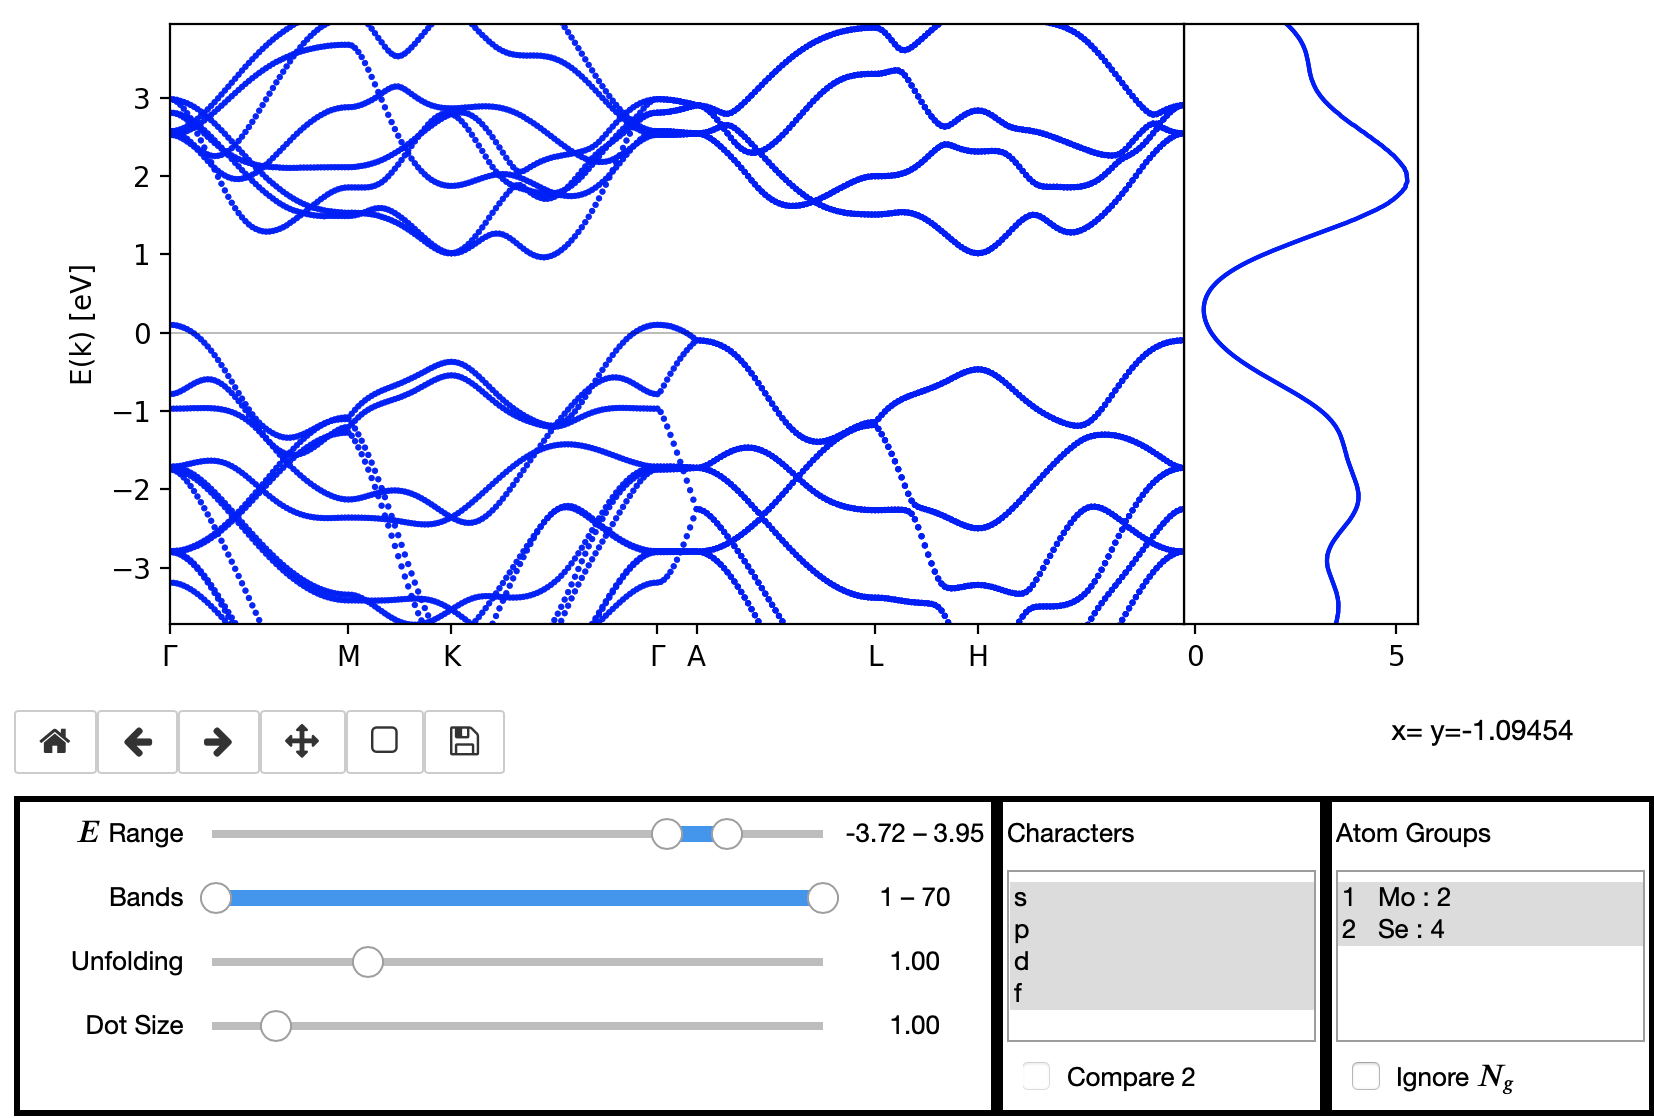
\includegraphics[width=1.0\textwidth]{data/screen1.png} 
    \end{figure}
\end{frame}

\begin{frame}[plain]
    \frametitle{Web GUI Demonstration}
    \begin{figure}
        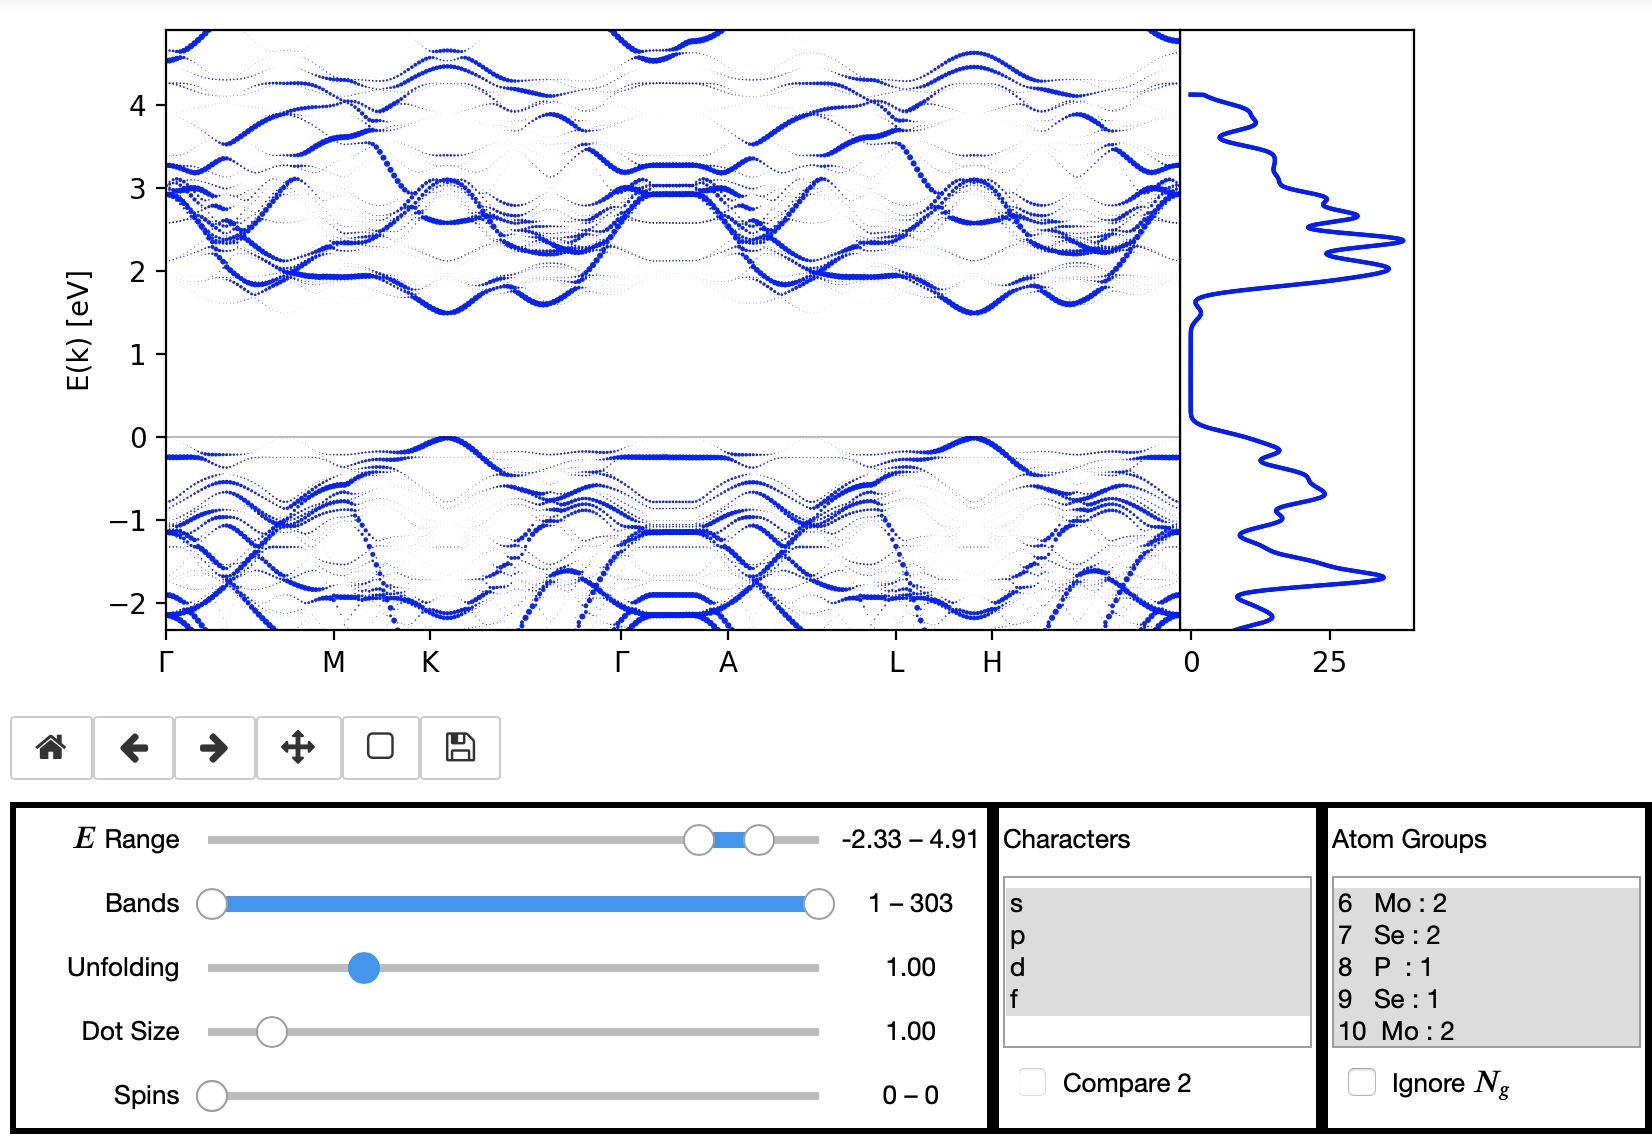
\includegraphics[width=1.0\textwidth]{data/screen2.png} 
    \end{figure}
\end{frame}

\begin{frame}[plain]
    \frametitle{Web GUI Demonstration}
    \begin{figure}
        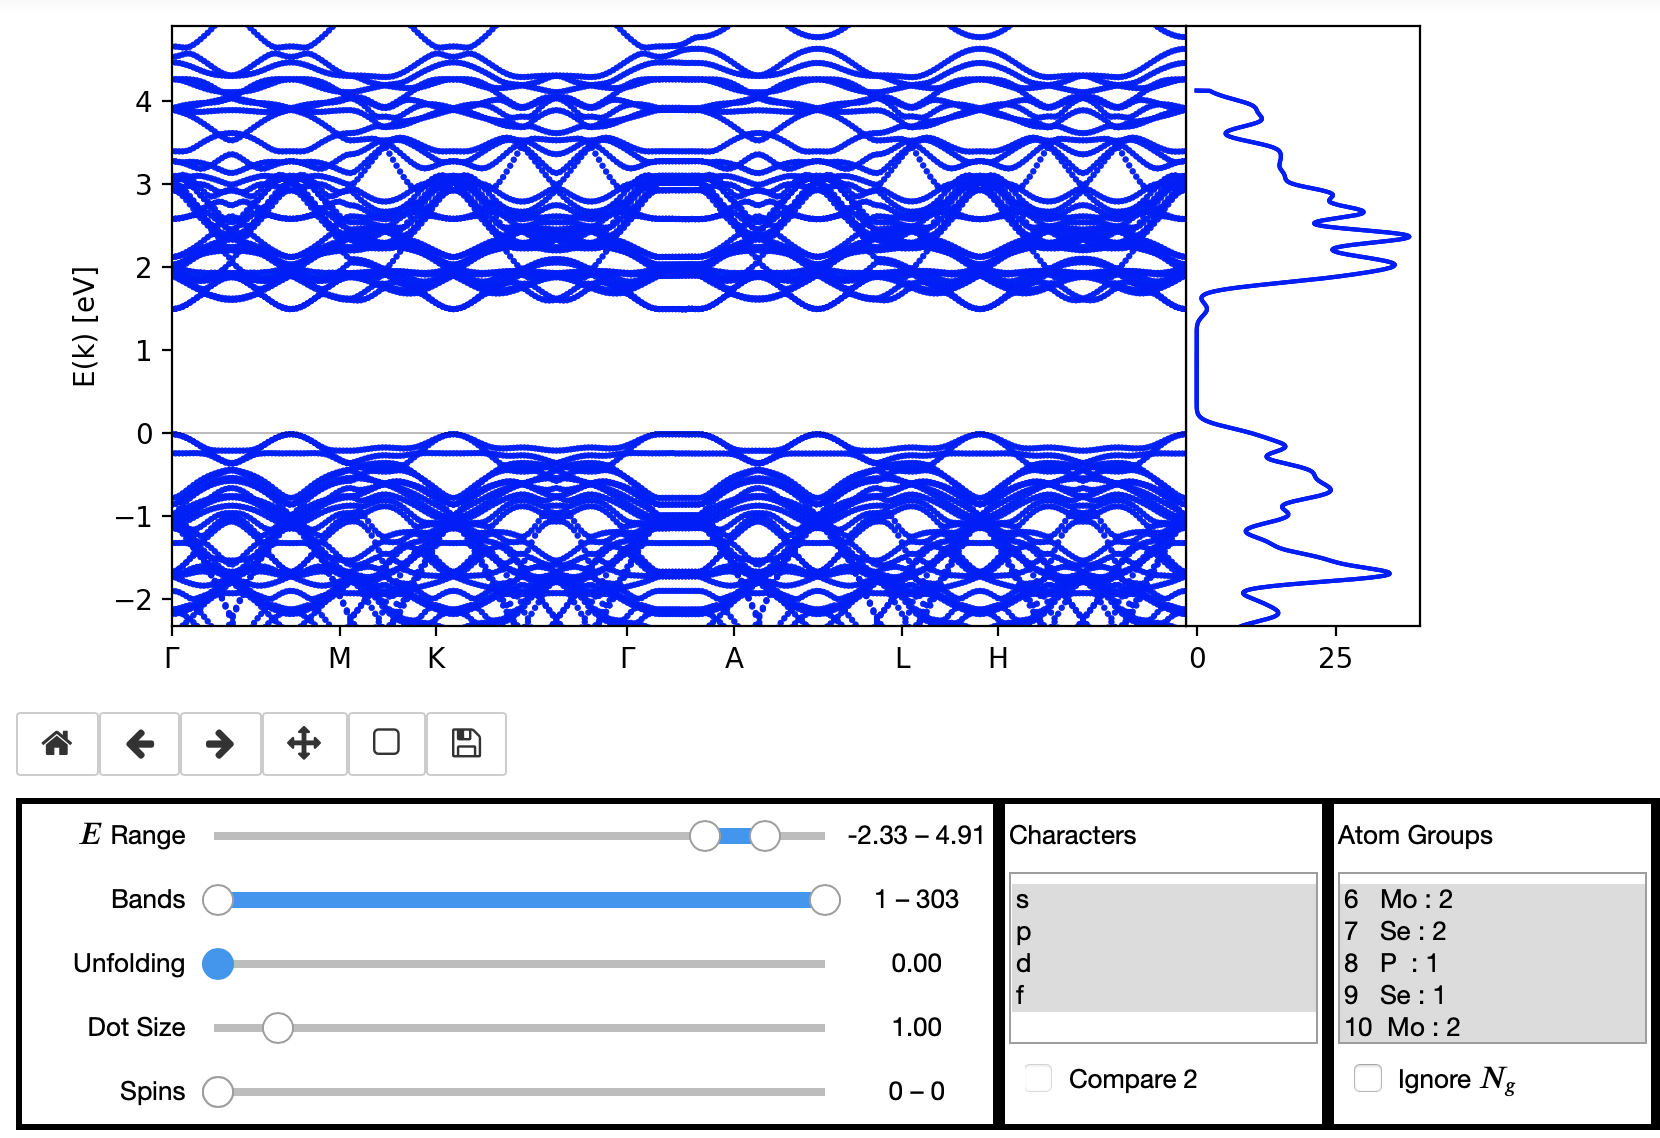
\includegraphics[width=1.0\textwidth]{data/screen3.png} 
    \end{figure}
\end{frame}

\begin{frame}\frametitle{Effective mass and group velocity:}
\begin{itemize}

\item Derived Quantities:

    \item Effective mass, that an electon in a crystal appears to have compared to a free electron (due to interactions in the solid)
    $m^{*} = \hbar^2  \left(\frac{\partial^2E(k)}{\partial k^2}\right)^{-1}$
    \
    \item Group velocity:
    $v_{G}(\vec{k}) = \frac{1}{\hbar}\frac{\partial E(\vec{k})}{\partial \vec{k}}$

    
    \item Problem: sparse k-Point mesh, but periodic bandstructure
    \item Idea: Using FFT to compute accurate derivates:
    \newline $\Leftrightarrow$ Differentiate a finite Fourier series
    \newline $f^{(n)}(x) = \mathcal{F}^{-1}\left((ik)^n\mathcal{F}(f(x))\right)$
\end{itemize}
\end{frame}

\begin{frame}
\begin{figure}
   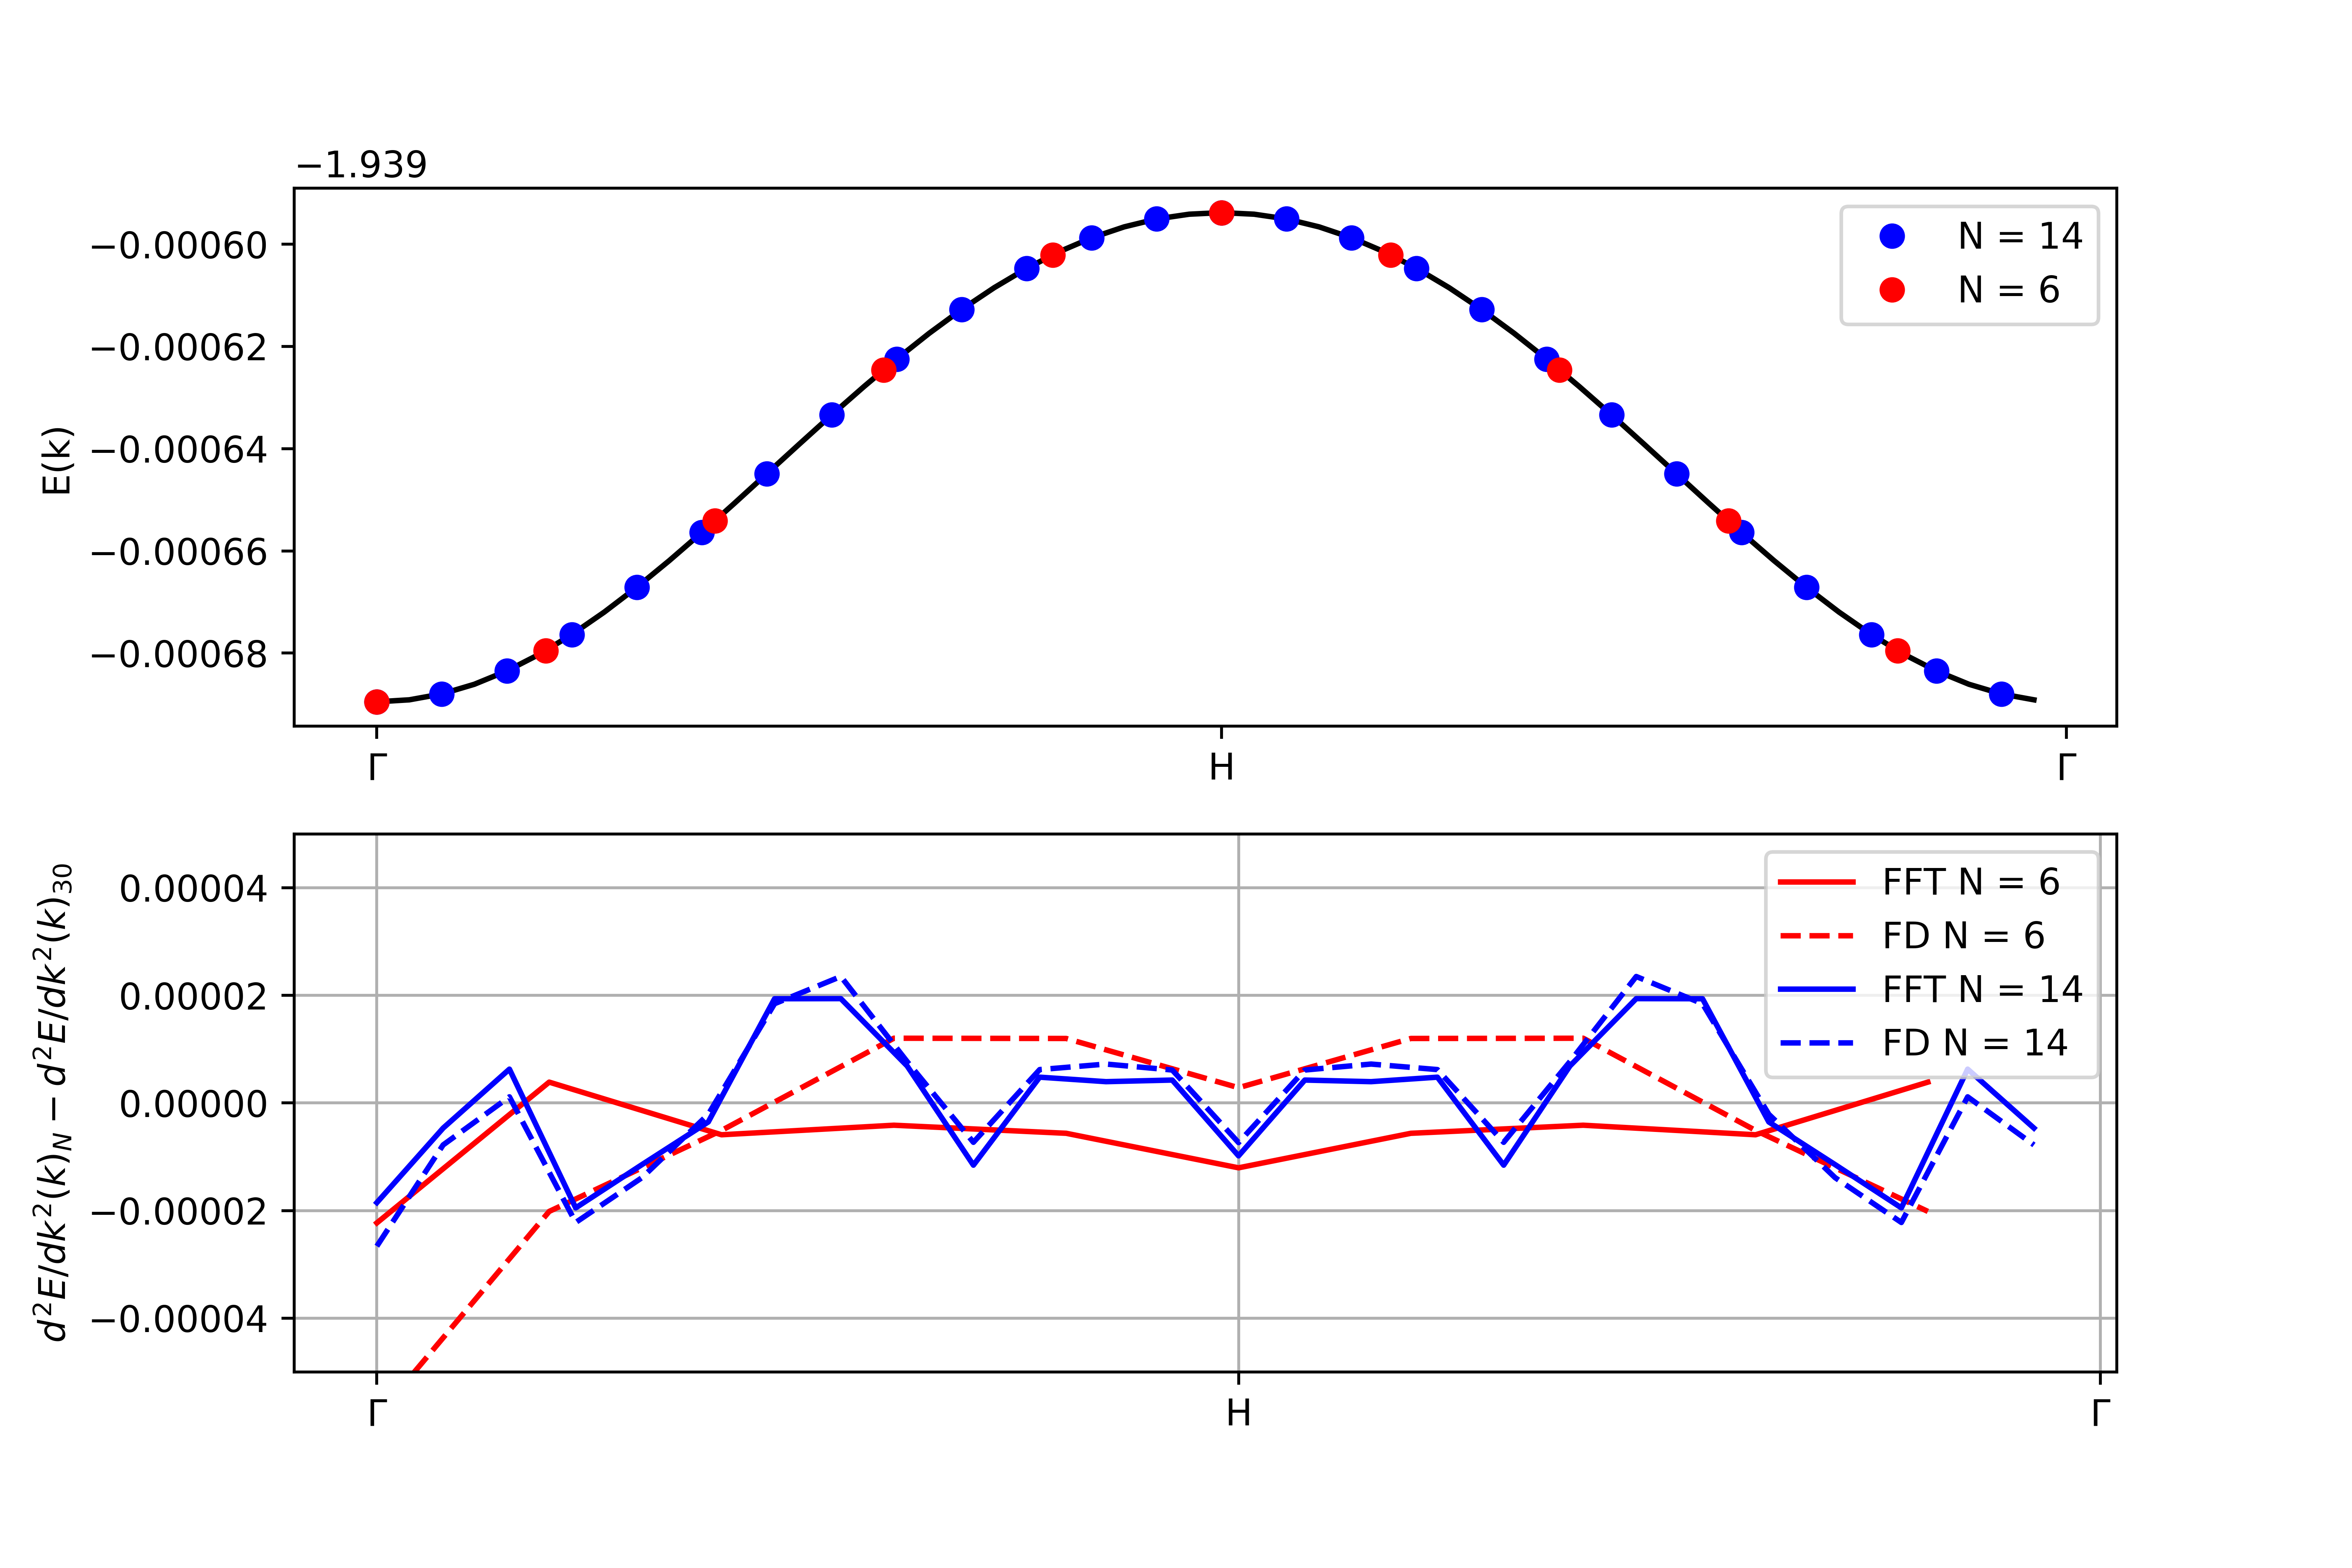
\includegraphics[width=1.0\linewidth]{data/diff_compare.png}
\end{figure}
\end{frame}




%% It is just an empty TeX file.
%% Write your code here.

\section{Conclusion} 


\end{document}
%%% Local Variables:
%%% mode: latex
%%% TeX-master: t
%%% End:
